\section{Базовый алгоритм}
Базовым алгоритмом в данной задаче является метод частичных наименьших квадратов (далее PLS).
Метод PLS относится к классу методов проекции на подпространства, которые предполагают поиск собственного базиса с последующим выбором в нем некоторого количества собственных векторов. Другие методы проекции на подпространства включают в себя метод главных компонент, линейный дискриминантный анализ и канонический корреляционный анализ. 

Метод PLS выгодно отличает то, что он позволяет одновременно выявлять скрытые связи между входными данными и аппроксимировать их. Более того, существуют реализации метода PLS, позволяющие построить регрессионную модель, описывающую зависимость между входными данными. 
Метод  PLS позволяет выделить из исходных данных компоненты, между которыми существует ковариационная связь. На основе этих компонент может быть построена модель регрессии. Такой подход позволяет не только существенно снизить вычислительные затраты, но и значительно улучшить точность модели по сравнению с линейной регрессией, построенной с помощью метода наименьших квадратов. 


\section{Базовый эксперимент}
Для проведения эксперимента, из данных электрокортикограммы были выделены частоты сигналов. Выходные данные~--- трехмерные координаты движения руки обезьяны. Полученные данные были разделены на обучающую и контрульную выборки в отношении два к одному. На полученной выборке был обучен двухкомпонентный PLS. Результаты эксперемента представлены на рисунке~\ref{fig:baseAlgo}.
\begin{figure}
  \begin{center}
    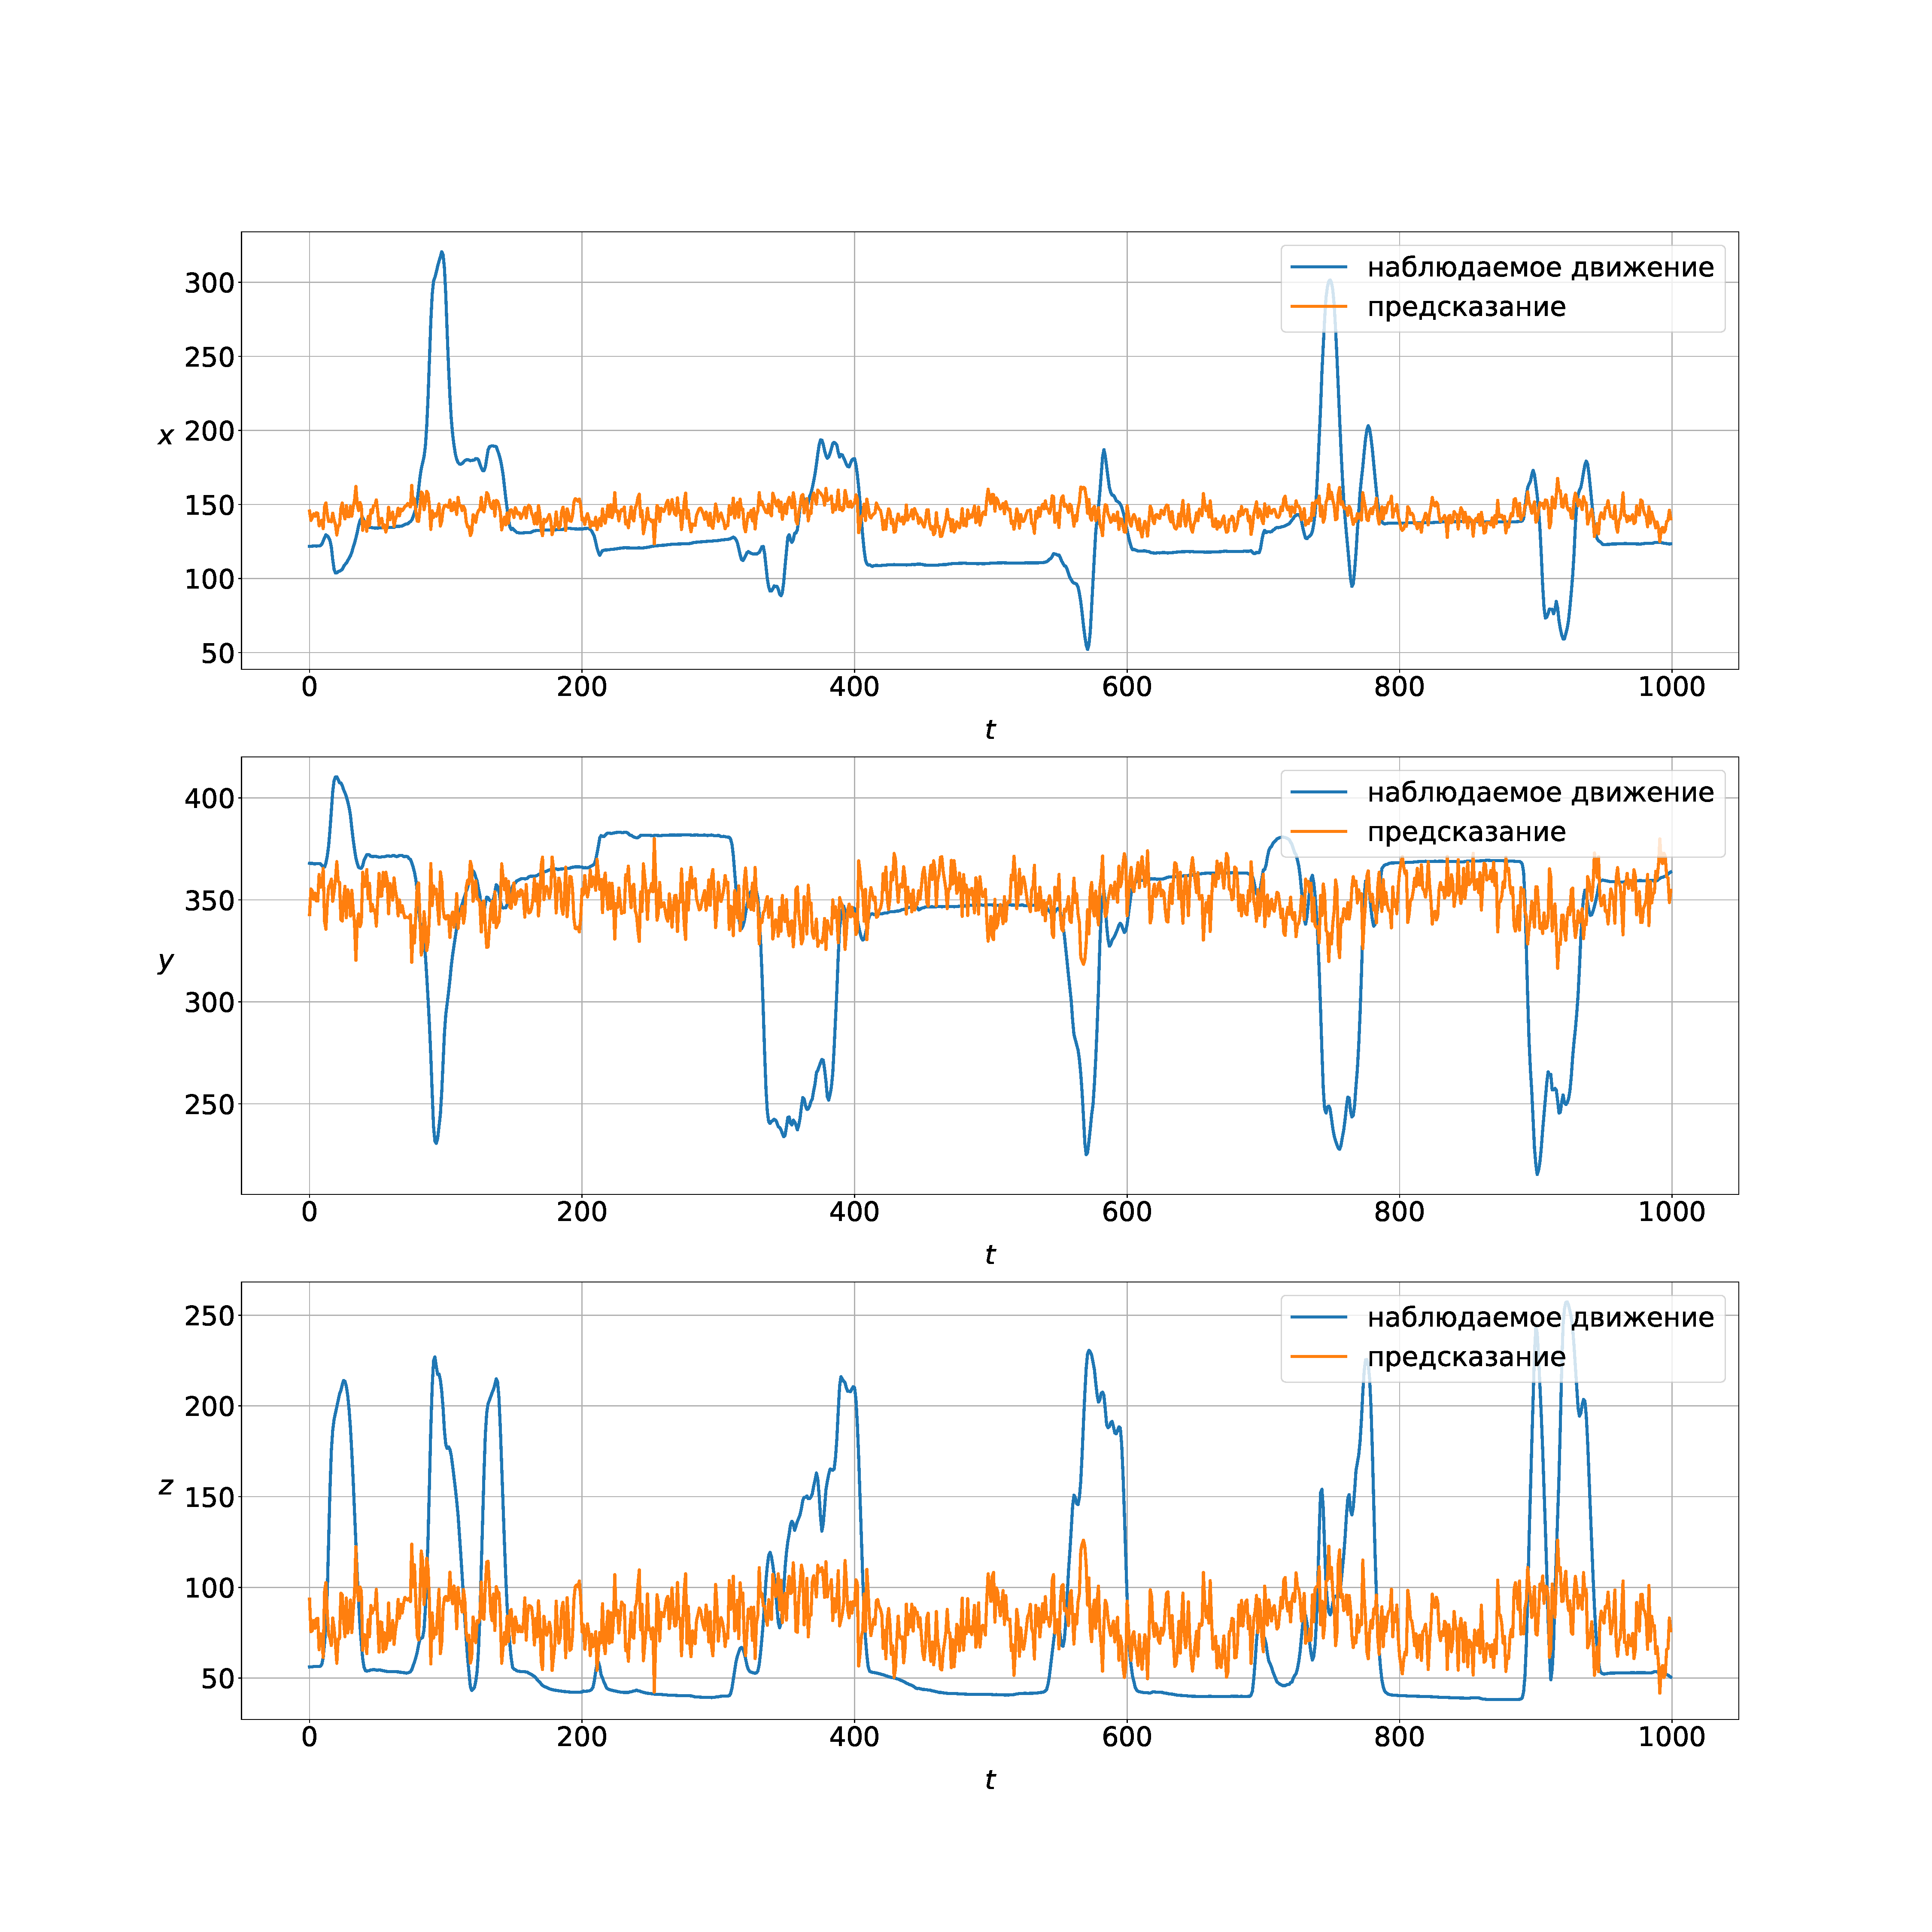
\includegraphics[width=\textwidth]{base_algo.pdf}
    \caption{Результаты эксперимента с базовым алгоритмом}
    \label{fig:baseAlgo}
  \end{center}
\end{figure}
На графике представлена зависимость координаты конечности от времени. Как видно из рисунка, базовый алгоритм довольно плохо справляется с поставленной задачей. Несмотря на то, что общий профиль пиков соблюдается, PLS не предсказывает острые пики, а также предсказывает флуктуации координаты во время, когда конечность почти не движется. В результате погрешность предсказания высока. Для борьбы с этим предлагается уменьшать размерность задачи, а значит и связанность данных.
